%!TEX root = ../main.tex
\chapter{Understanding the degradation of the energy resolution with timing cuts}
\label{appendix:eresdegrad}

To investigate and understand the degradation of the energy resolution with timing cuts, a simple complementary analysis has been done based on the CAN 028 \cite{CaN028}. This CALICE Analysis note presents a software compensation method to improve energy resolution using a correction factor derived from the knowledge of the electromagnetic and hadronic fraction in a shower on an event-by-event basis. It was found that the shape of energy density distributions is correlated with the calorimeter response. The goal of this study is to show that timing cuts favor high electromagnetic fraction events and reduces the correlation.

\section{Hit Energy spectra in HCAL}

Due to the high granularity of the HCAL in the ILD detector, a detailed study of hadronic showers is possible at the single cell level (hits). The hadronic calorimeter in ILD is of a non-compensating nature resulting in a higher response of the electromagnetic component of a hadronic shower to the hadronic response. The $\frac{e}{\pi}$ ratio is around 1.19. Because of this, hadron induced shower with a higher electromagnetic fraction will give a higher response and vice-versa. An example is shown in figure \ref{fig:Esum30_100ns}. $E_{mean}$ and $\sigma$ correspond to the mean of the distribution and RMS, respectively. The blue subsample can be identified to events reconstructed with $E_{reco} < E_{mean} - \sigma$ and the red one with $E_{reco} > E_{mean} + \sigma$. The corresponding hit energy spectrum is shown in figure \ref{fig:HitSpectra30_100ns}. This shows that the shape of the hit energy spectrum is related to the deposited energy.

\begin{figure}[htbp!]
  \centering
  \begin{subfigure}[t]{0.45\textwidth}
    \centering
    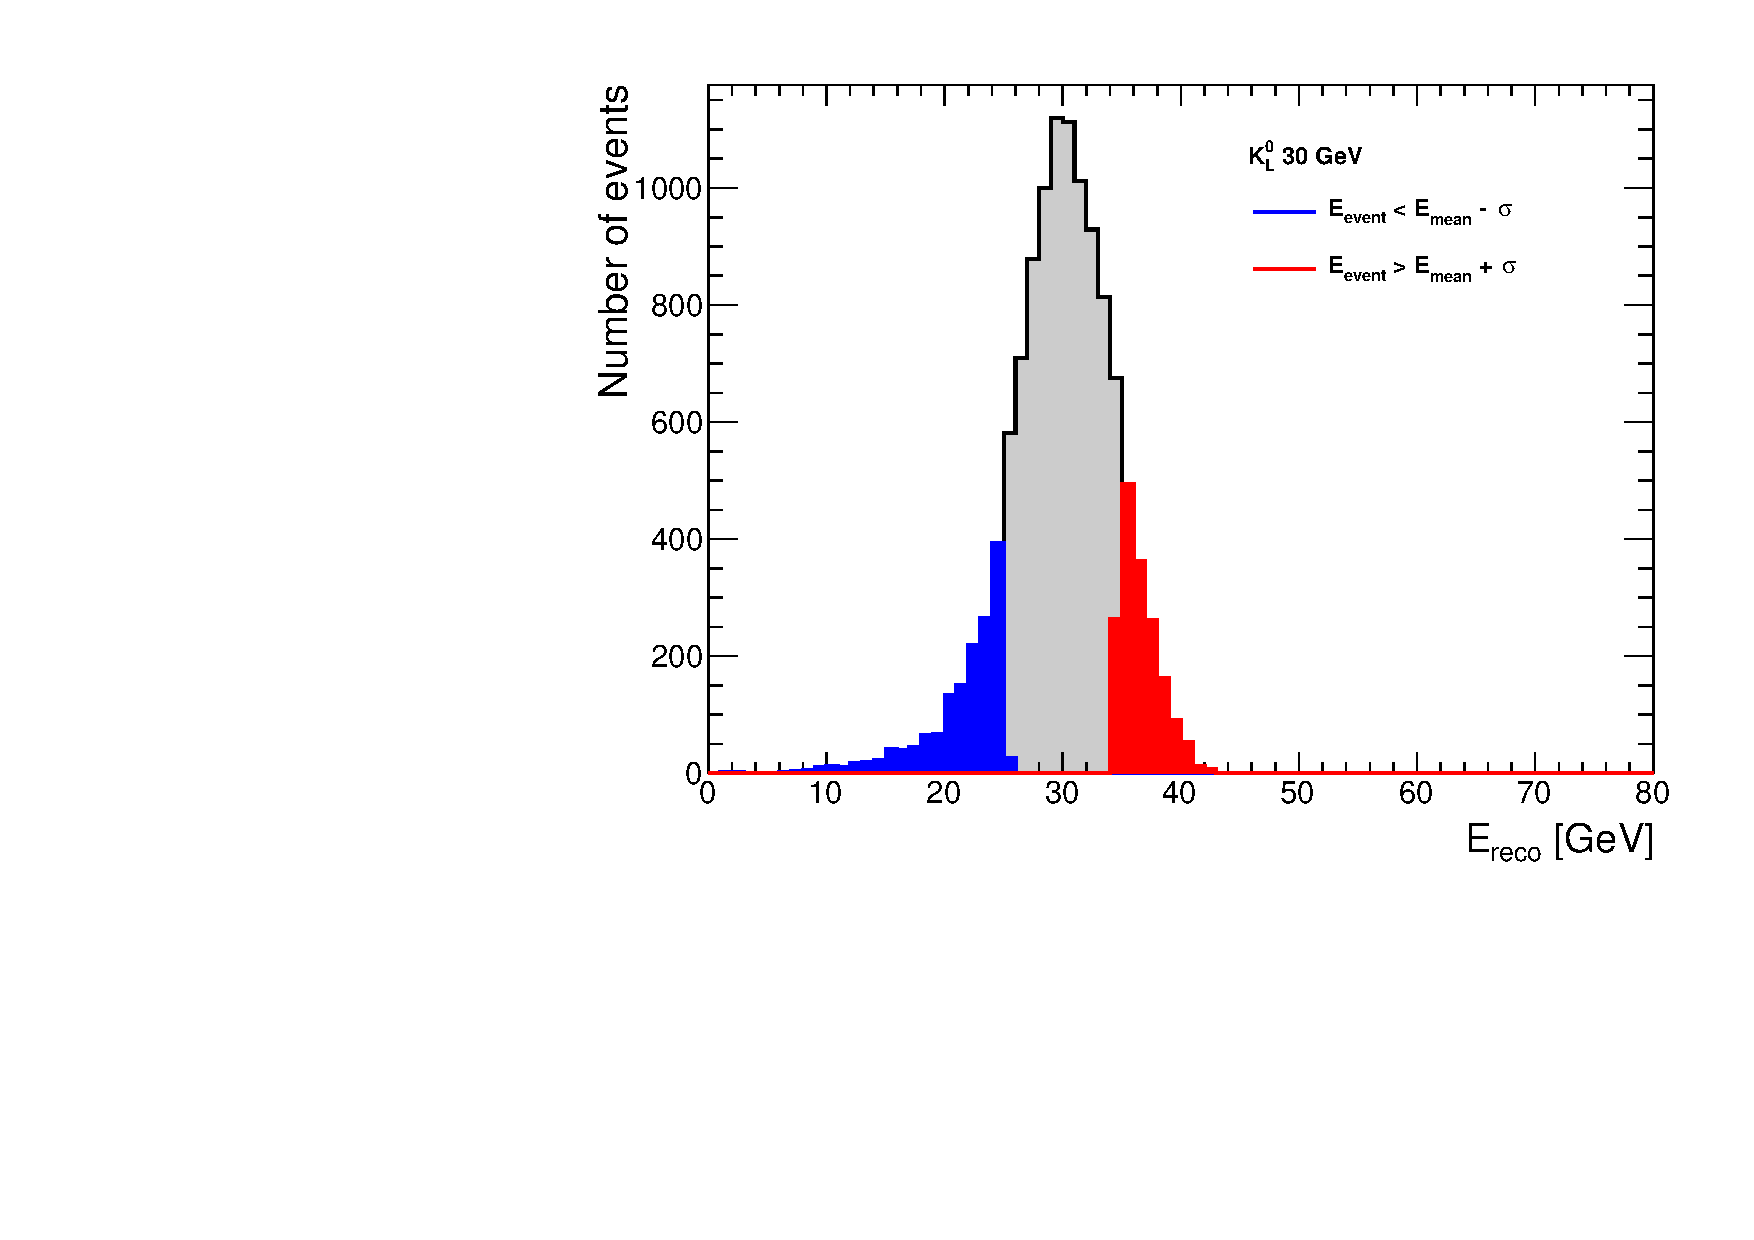
\includegraphics[width=1\linewidth]{../Thesis_Plots/ILD/AdditionalPlots/Plots/EnergySum_100ns_30GeV.pdf}
    \caption{} \label{fig:Esum30_100ns}
  \end{subfigure}
  \hfill
  \begin{subfigure}[t]{0.45\textwidth}
    \centering
    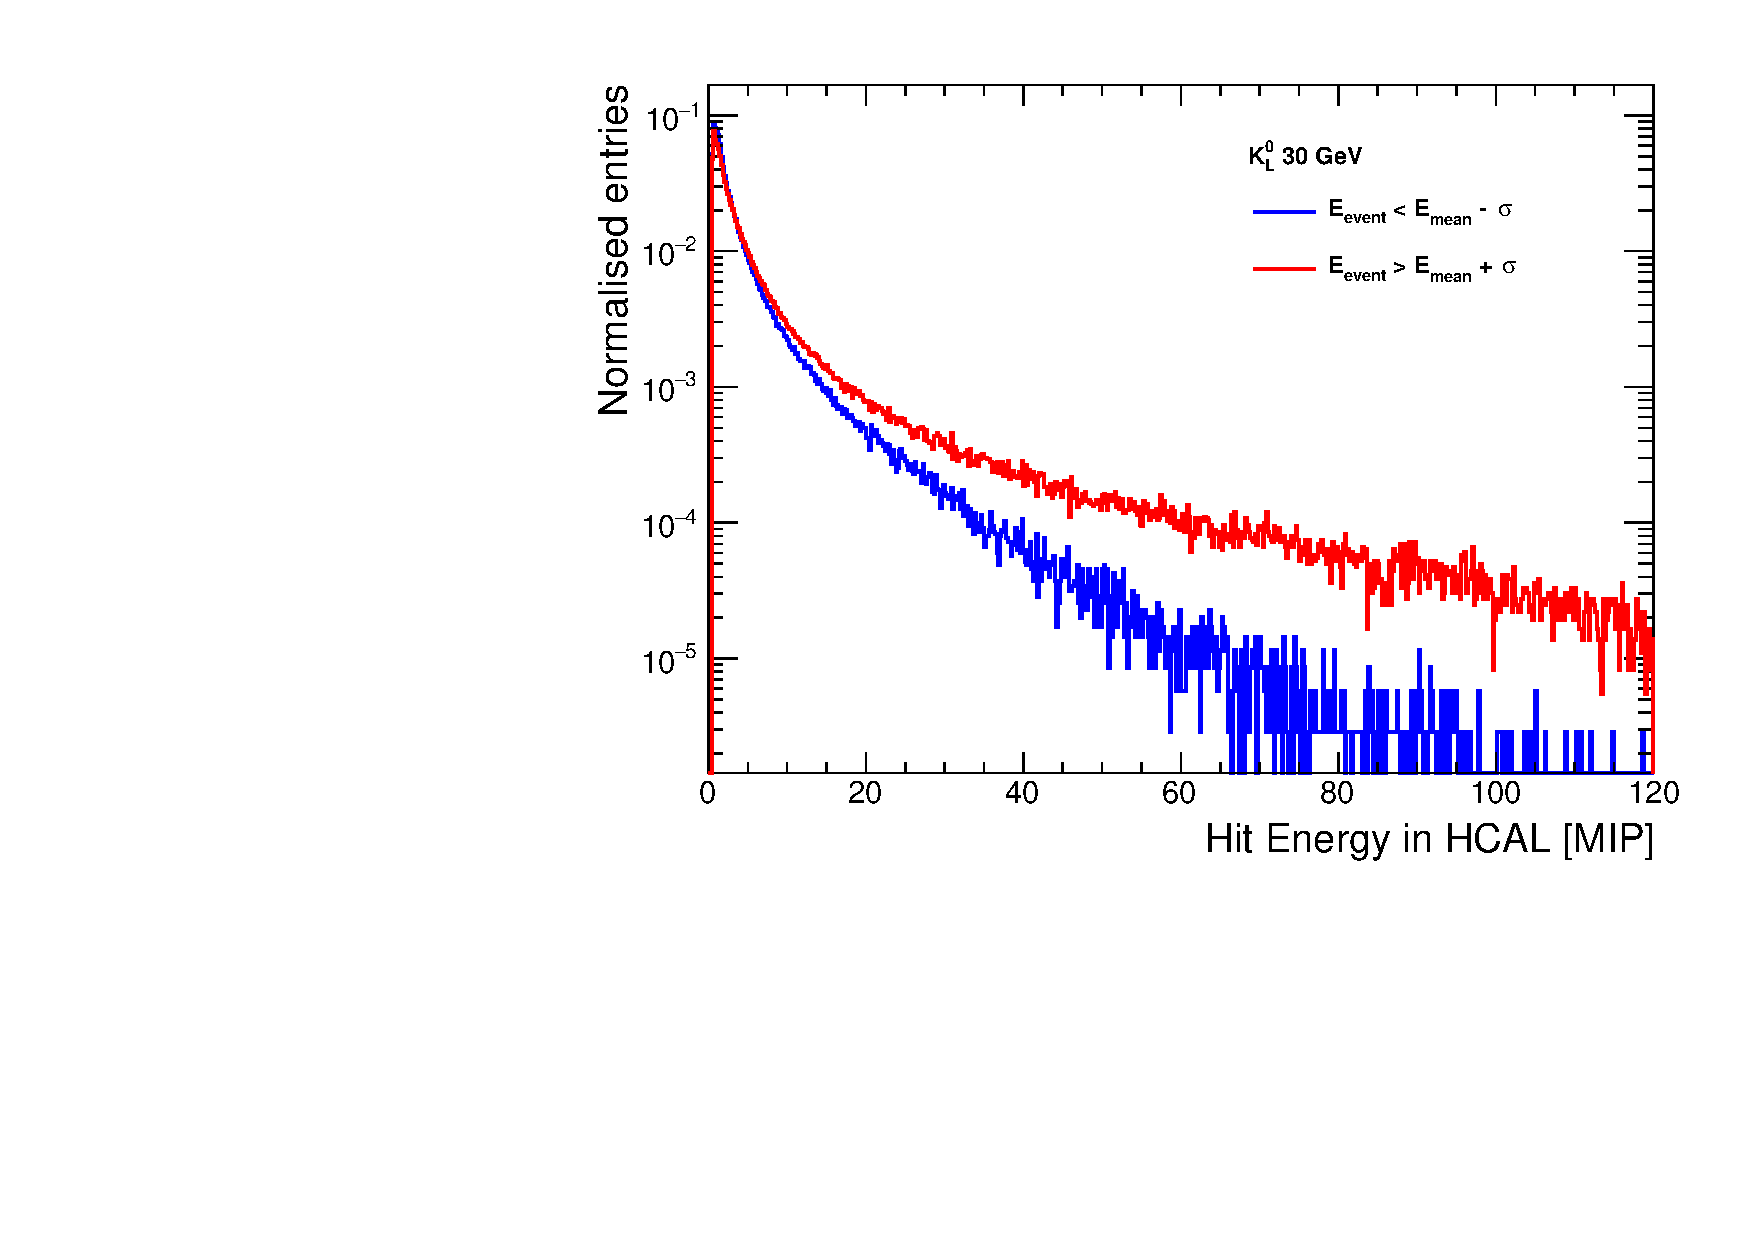
\includegraphics[width=1\linewidth]{../Thesis_Plots/ILD/AdditionalPlots/Plots/HitEnergySpectra_100ns_30GeV.pdf}
    \caption{} \label{fig:HitSpectra30_100ns}
  \end{subfigure}
  \caption{\subref{fig:Esum30_100ns}) Reconstructed energy distribution for 30 GeV kaons. \subref{fig:HitSpectra30_100ns}) Associated hit energy spectrum in the HCAL corresponding to subsamples with low (in blue) and high (in red) energy depositions.}
\end{figure}

Following the note, a quantitative probability $C_{i}^{lim}$ of the i-th event was obtained as follows:
\begin{equation}
  C_{i}^{lim} = \frac{N_{i}(e \leq e^{lim})}{N_{i}^{HCAL}}
\end{equation}

where $N_{i}(e \leq e^{lim})$ is the number of hits with energy $e \leq e^{lim}$ and $N_{i}^{HCAL}$ the number of hits in the HCAL. For events with a lower energy deposition (blue spectrum), they have a higher $C_{i}^{lim}$ probability. The value of $e^{lim}$ is in an interval of 3 to 5 MIPs and was observed for the intersection of hit energy spectra for kaons betweeen 10 and 80 GeV as an example is shown in figure \ref{fig:HitSpectra30_Zoom_100ns}.

\begin{figure}[htbp!]
  \centering
  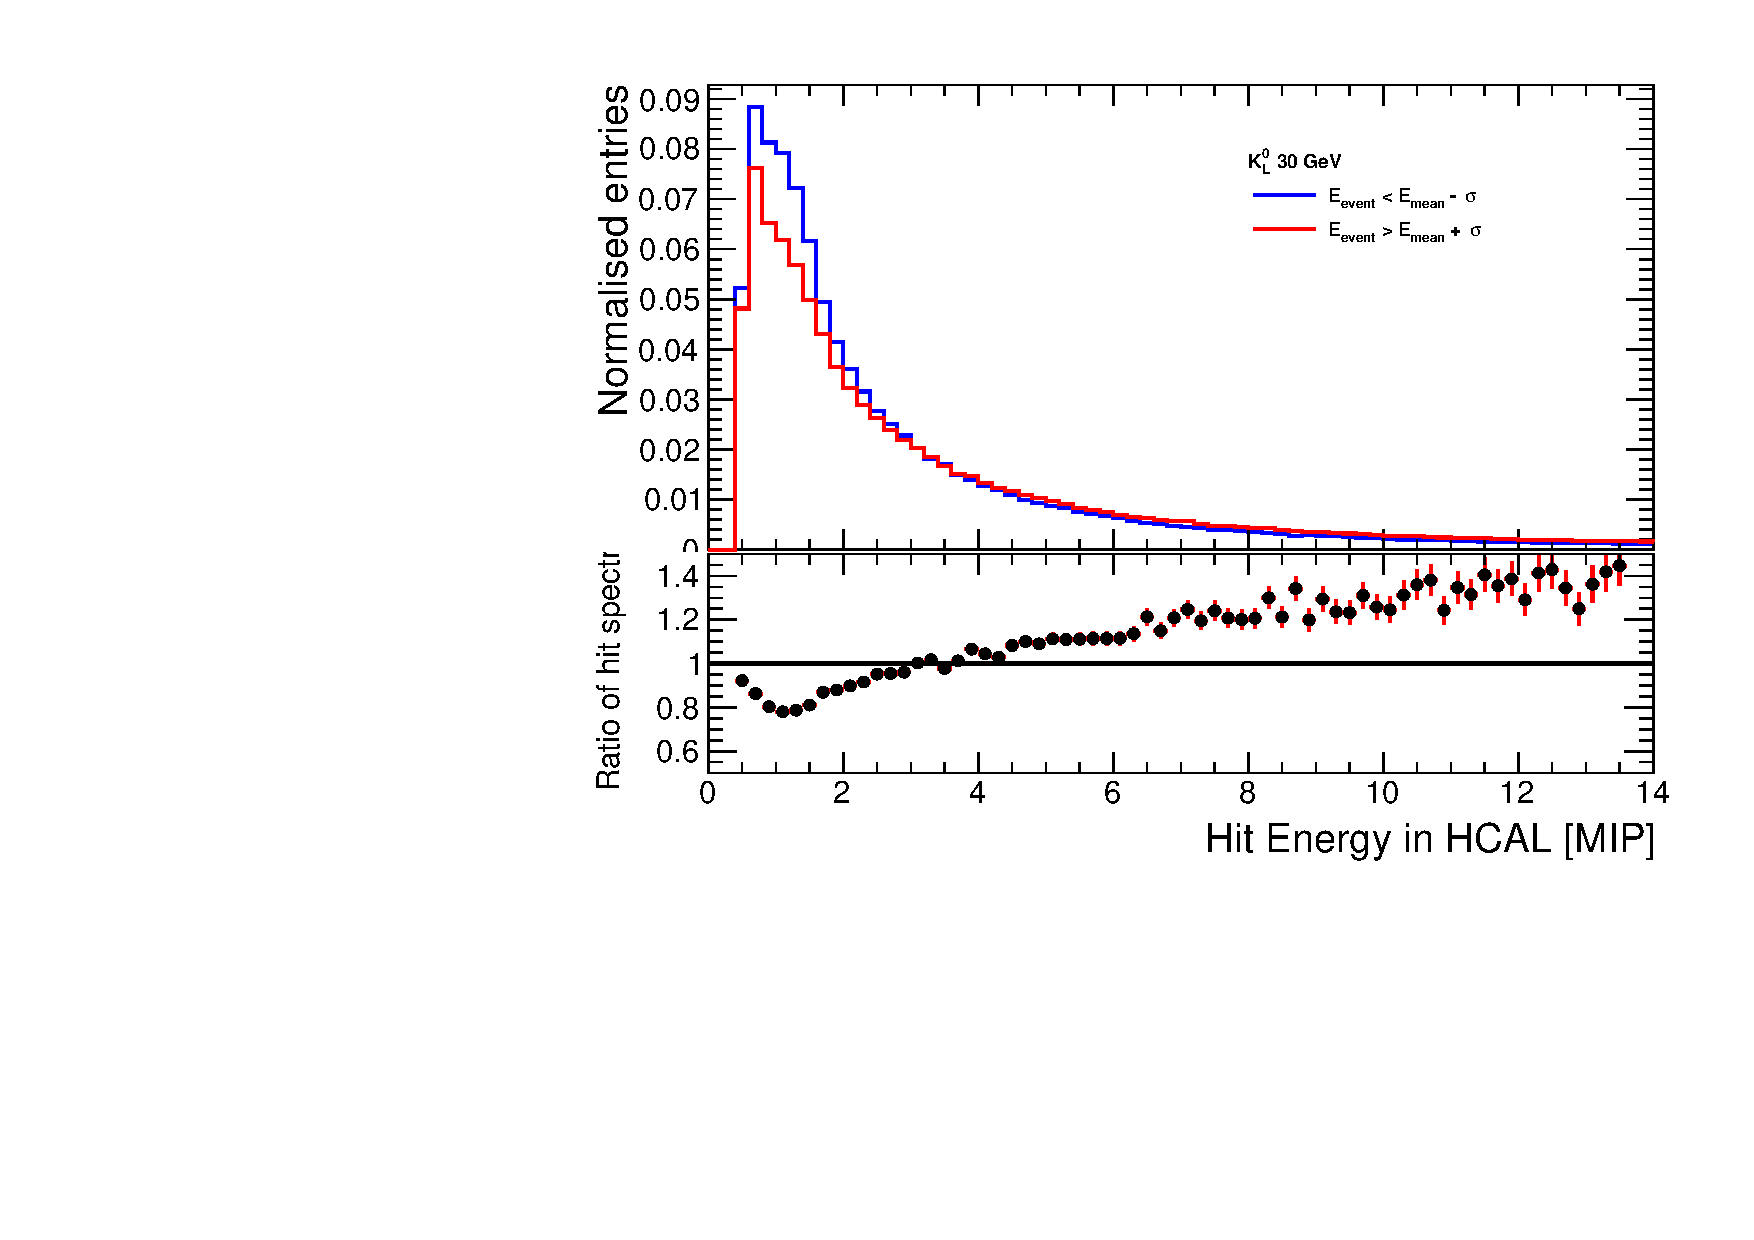
\includegraphics[width=0.7\linewidth]{../Thesis_Plots/ILD/AdditionalPlots/Plots/HitEnergySpectra_Zoom_100ns_30GeV.pdf}
  \caption{The top plot shows the hit energy spectrum in the HCAL for 30 GeV kaons for the subsample low (blue) and high (red) of energy depositions. The bottom plot shows the ratio of the red to the blue spectrum.} \label{fig:HitSpectra30_Zoom_100ns}
\end{figure}

The distribution of $C^{lim}$ for different values of $e^{lim}$ are shown in figures \ref{fig:CLim10_100ns} and \ref{fig:CLim80_100ns} for 10 GeV and 80 GeV kaons. One can see that the distributions get narrower with increasing $e^{lim}$. A higher value of $e^{lim}$ results with more events with a value of $C^{lim}$ close to 1. For this analysis, a value of 3.5 MIP was chosen for $e^{lim}$.

\begin{figure}[htbp!]
  \centering
  \begin{subfigure}[t]{0.45\textwidth}
    \centering
    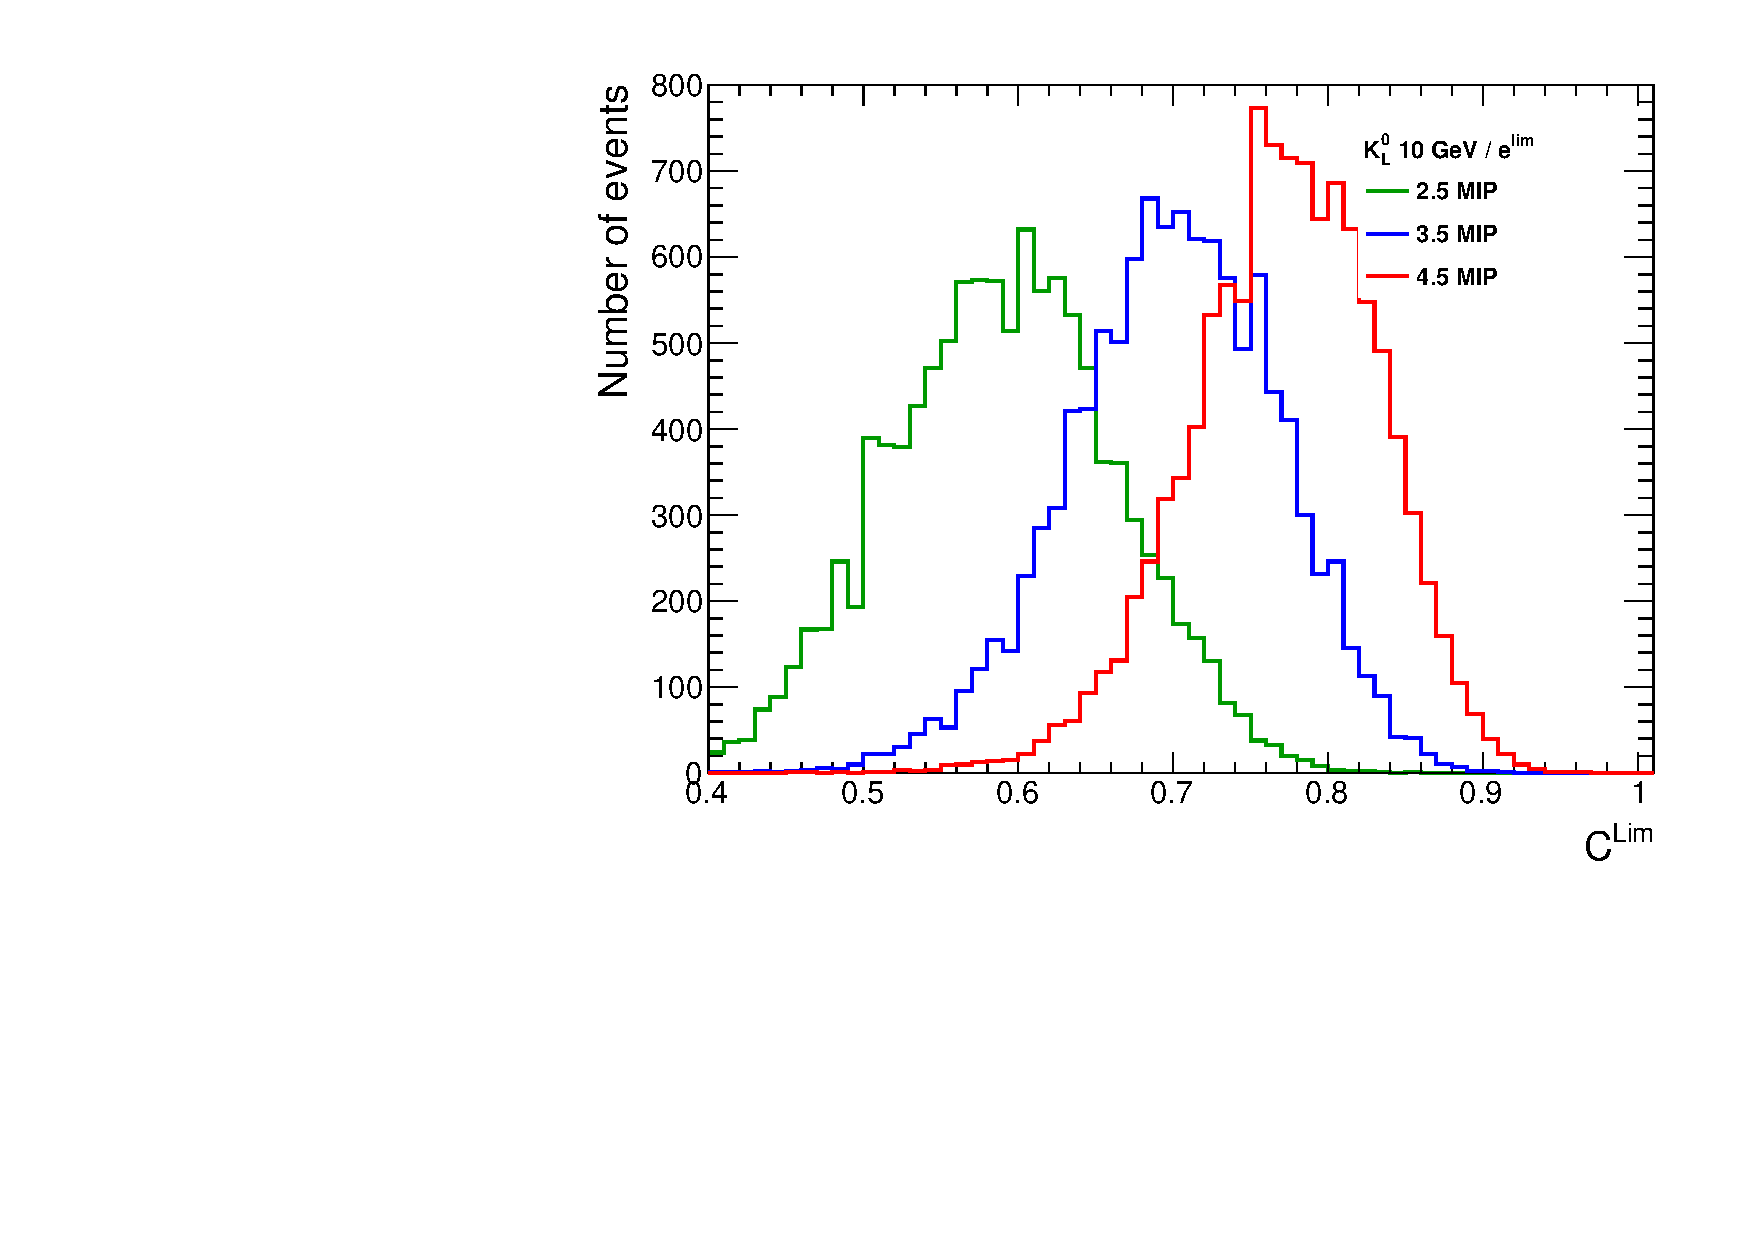
\includegraphics[width=1\linewidth]{../Thesis_Plots/ILD/AdditionalPlots/Plots/CLim_100ns_10GeV.pdf}
    \caption{10 GeV.} \label{fig:CLim10_100ns}
  \end{subfigure}
  \hfill
  \begin{subfigure}[t]{0.45\textwidth}
    \centering
    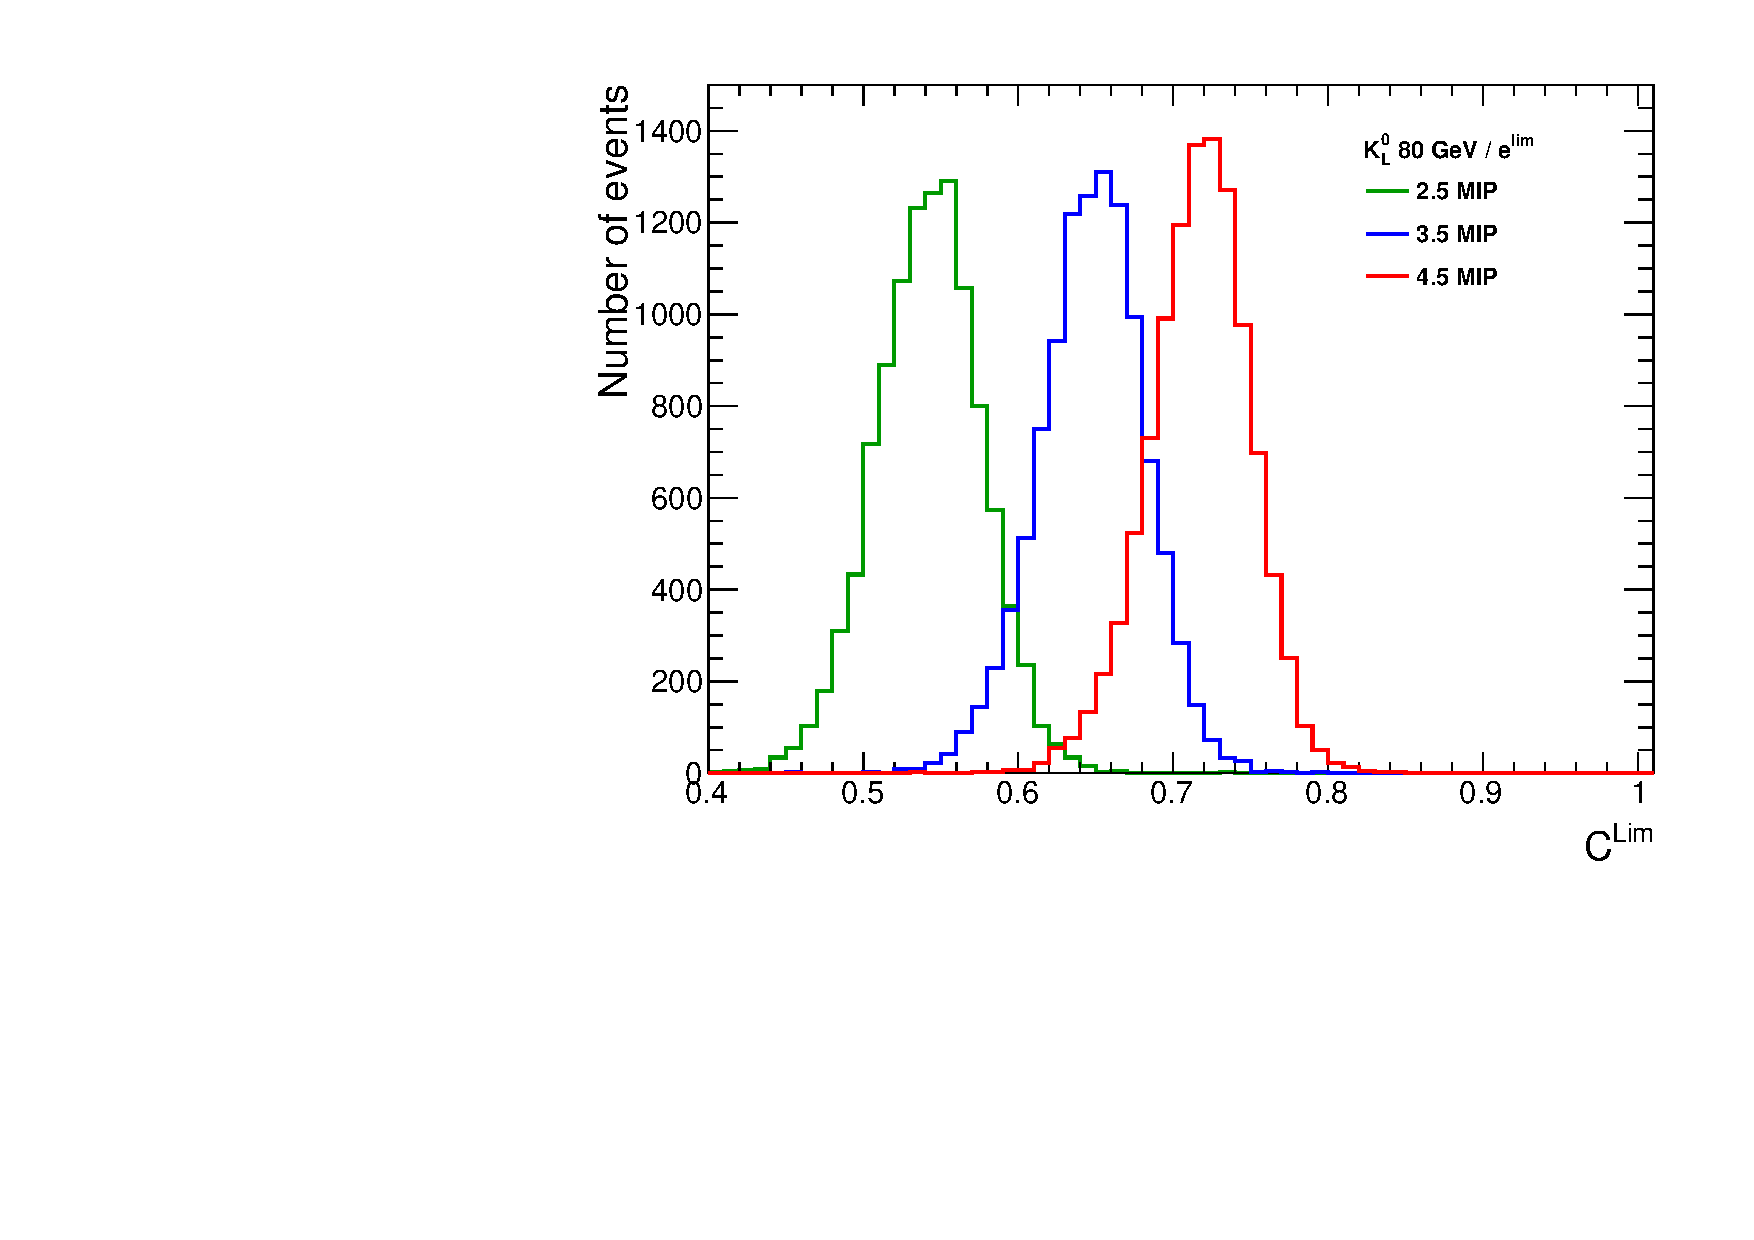
\includegraphics[width=1\linewidth]{../Thesis_Plots/ILD/AdditionalPlots/Plots/CLim_100ns_80GeV.pdf}
    \caption{80 GeV.} \label{fig:CLim80_100ns}
  \end{subfigure}
  \caption{\subref{fig:CLim10_100ns}) Distributions of $C^{lim}$ for different values of $e^{lim}$ for 10 GeV kaons. \subref{fig:CLim80_100ns}) Distributions of $C^{lim}$ for different values of $e^{lim}$ for 80 GeV kaons.}
\end{figure}

Similarly another variable $C_{i}^{av}$ was calculated as follows:
\begin{equation}
  C_{i}^{av} = \frac{N_{i}(e \leq e_{i}^{av})}{N_{i}^{HCAL}}
\end{equation}

where $N_{i}(e \leq e^{av})$ is the number of hits with energy $e \leq e_{i}^{av}$, $e_{i}^{av}$ is the mean of the energy spectrum of the i-th event and $N_{i}^{HCAL}$ the number of hits in the HCAL. The ratio of $C_{i}^{lim}$ and $C_{i}^{av}$ is calculated for each event and appears inversely correlated to the deposited energy in the HCAL $E_i^{HCAL}$. It is shown in figures \ref{fig:EhcalCLimCav10_100ns} and \ref{fig:EhcalCLimCav80_100ns}.

\begin{figure}[htbp!]
  \centering
  \begin{subfigure}[t]{0.45\textwidth}
    \centering
    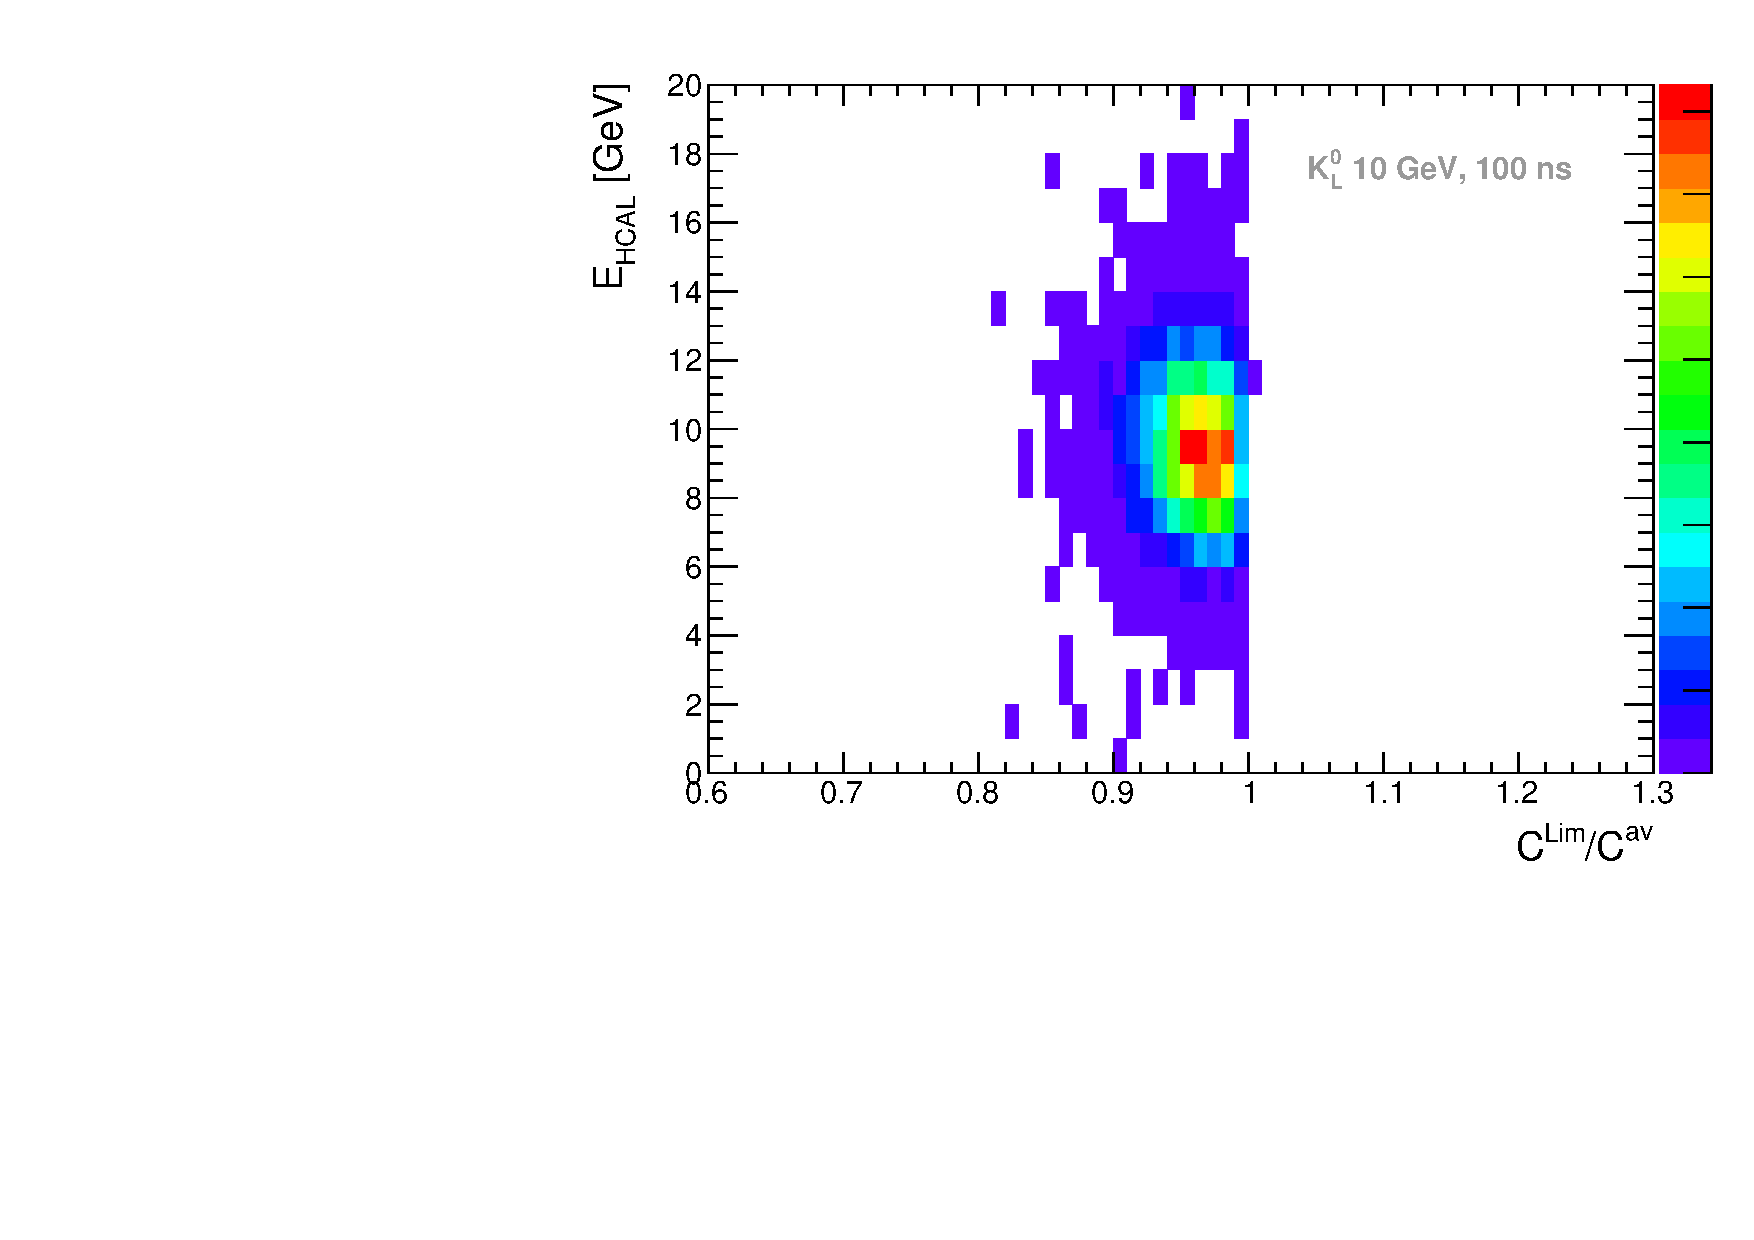
\includegraphics[width=1\linewidth]{../Thesis_Plots/ILD/AdditionalPlots/Plots/EhcalCLimCav_100ns_10GeV.pdf}
    \caption{10 GeV.} \label{fig:EhcalCLimCav10_100ns}
  \end{subfigure}
  \hfill
  \begin{subfigure}[t]{0.45\textwidth}
    \centering
    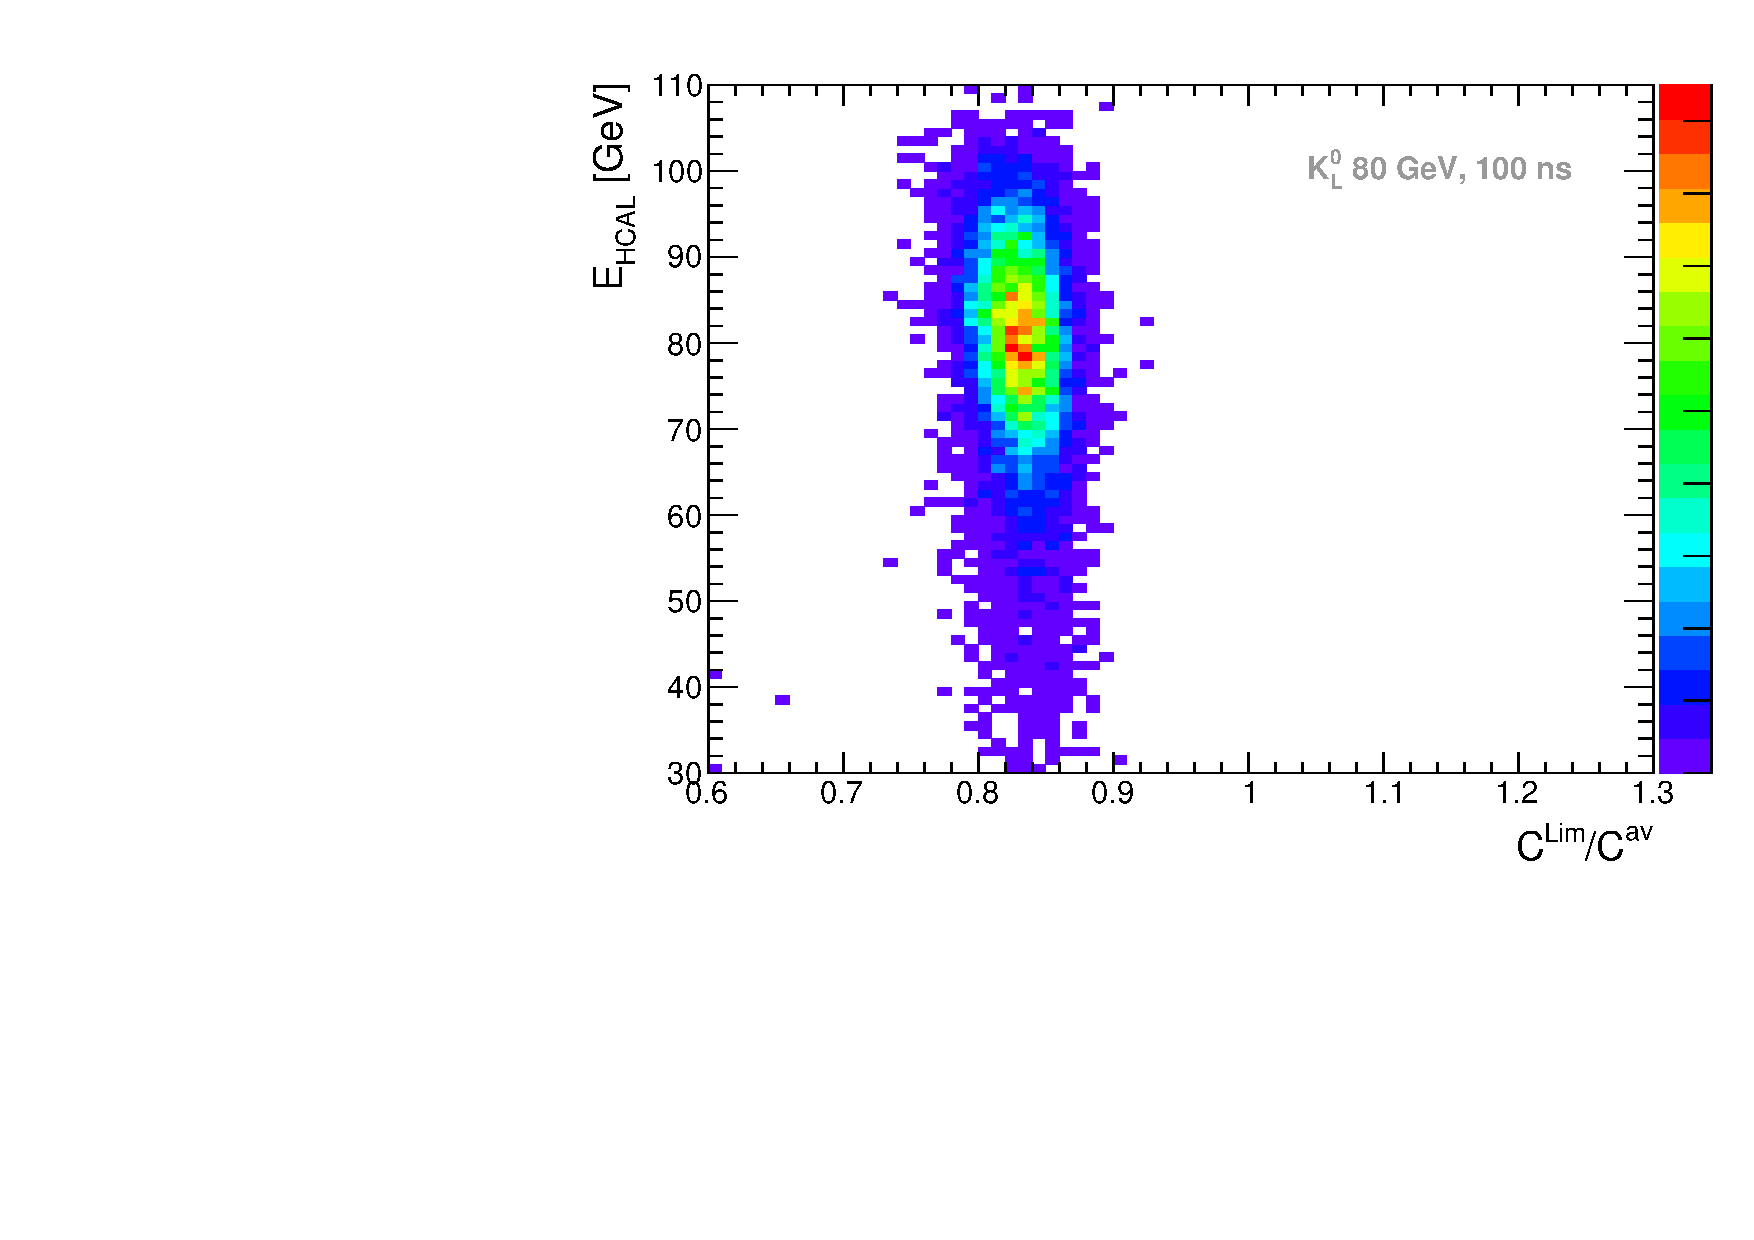
\includegraphics[width=1\linewidth]{../Thesis_Plots/ILD/AdditionalPlots/Plots/EhcalCLimCav_100ns_80GeV.pdf}
    \caption{80 GeV.} \label{fig:EhcalCLimCav80_100ns}
  \end{subfigure}
  \caption{\subref{fig:EhcalCLimCav10_100ns}) Correlation between the energy deposited in the HCAL for 10 GeV kaons and $C^{lim}$/$C^{av}$ for $e^{lim}$ = 3.5 MIPs. \subref{fig:EhcalCLimCav80_100ns}) Correlation between the energy deposited in the HCAL for 80 GeV kaons and $C^{lim}$/$C^{av}$ for $e^{lim}$ = 3.5 MIPs.}
\end{figure}

The inverse correlation is much stronger for higher kaon energies and becomes weaker with lower energies. By looking at the figure \ref{fig:CLimCav_100ns}, it appears that fluctuations are stronger at lower energies and $C^{lim}$/$C^{av}$ is energy dependent.

\begin{figure}[htbp!]
  \centering
  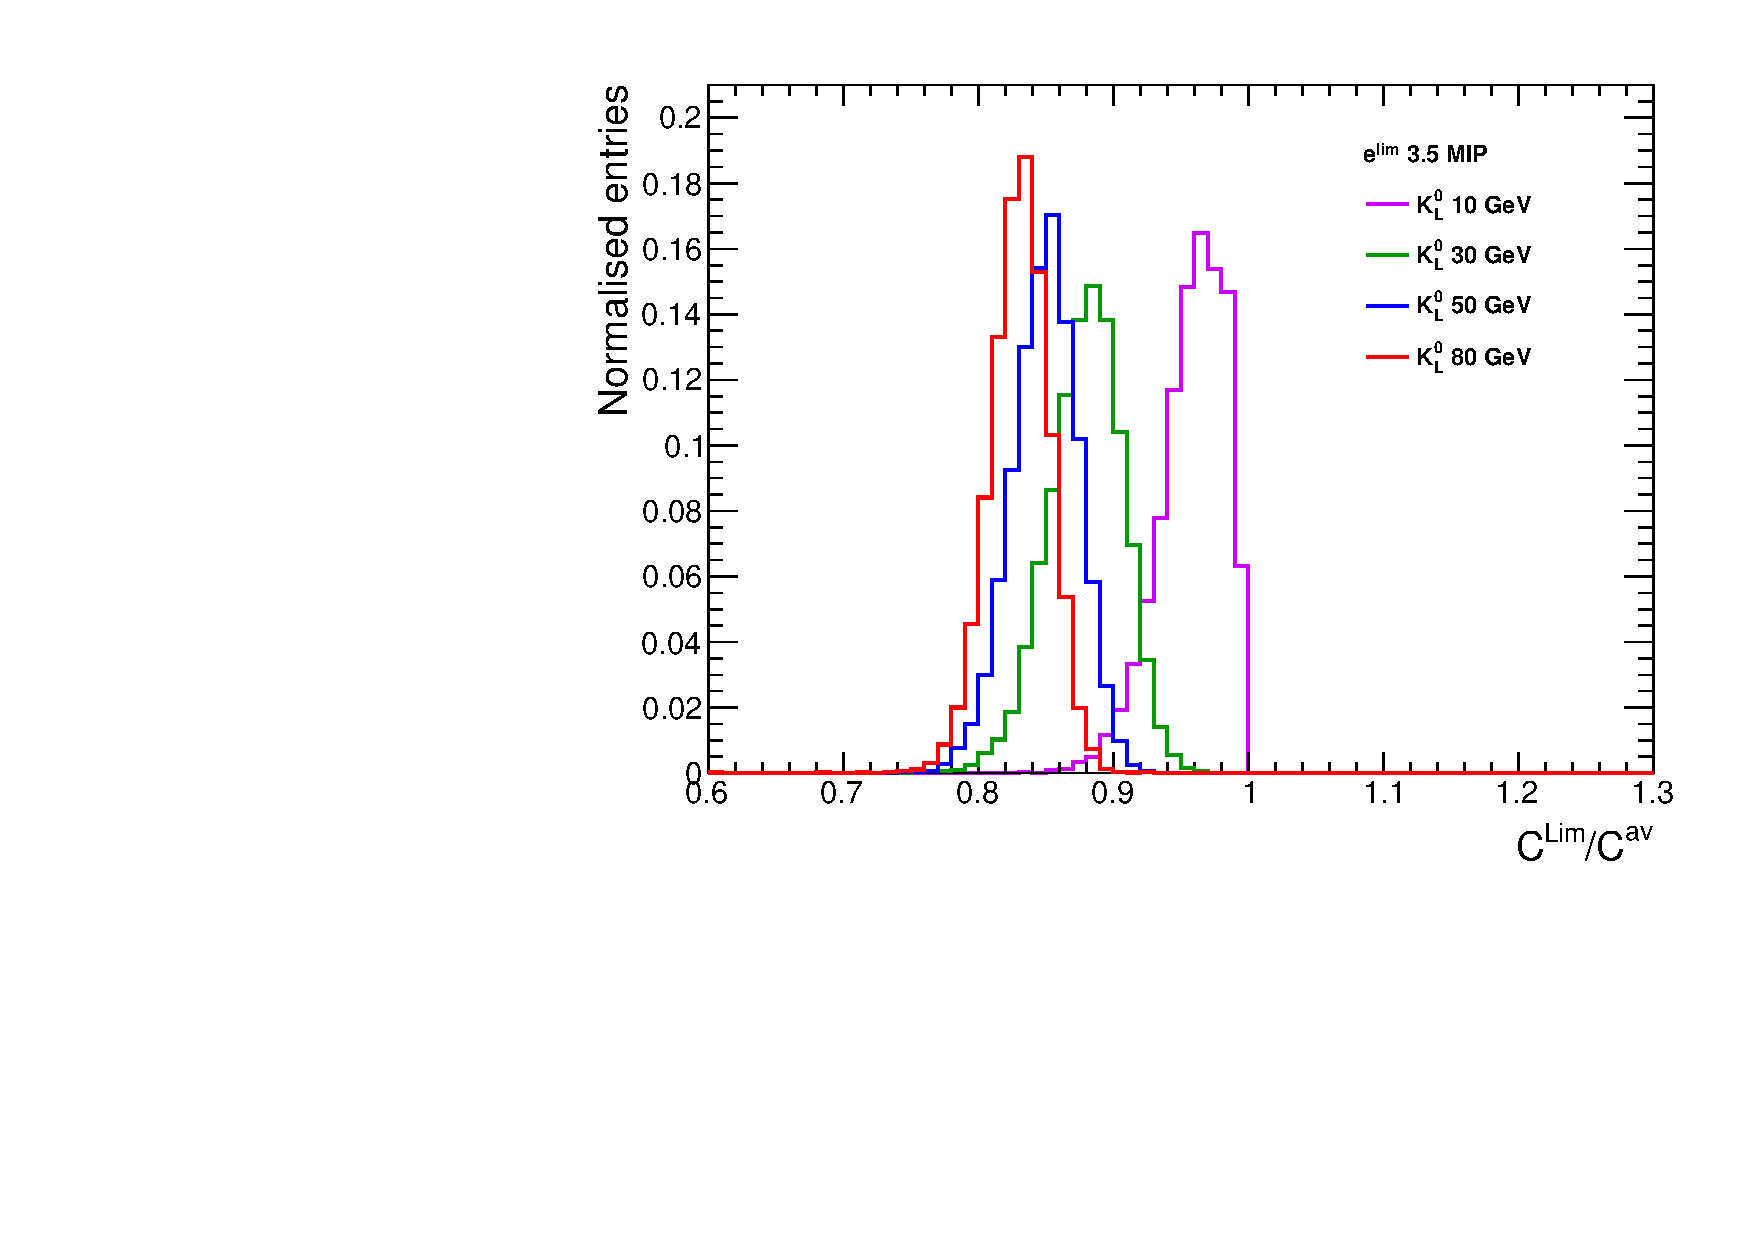
\includegraphics[width=0.7\linewidth]{../Thesis_Plots/ILD/AdditionalPlots/Plots/CLimCav_100ns_SeveralEnergies.pdf}
  \caption{Distributions of $C^{lim}$/$C^{av}$ for different kaon energies.} \label{fig:CLimCav_100ns}
\end{figure}

In a next step, timing cut will be applied and a comparison with these results will be done. It is believed that timing cuts will have an effect of reducing the inverse correlation of $C^{lim}$/$C^{av}$ with the energy deposited as fluctuation are cut down by timing cuts thus would favor higher electromagnetic fraction hadronic showers.

\section{Influence of timing cuts on hit energy spectra in HCAL}

A first check was performed on the shape of the hit spectra in the HCAL with different timing cuts. The figure \ref{fig:HitSpectra80_timingcuts} shows the hit spectra for 80 GeV kaons with a timing cut of 100, 5 and 1 ns. The green line in the bottom plot represents the value of $e^{lim}$ = 3.5 MIPs.

\begin{figure}[htbp!]
  \centering
  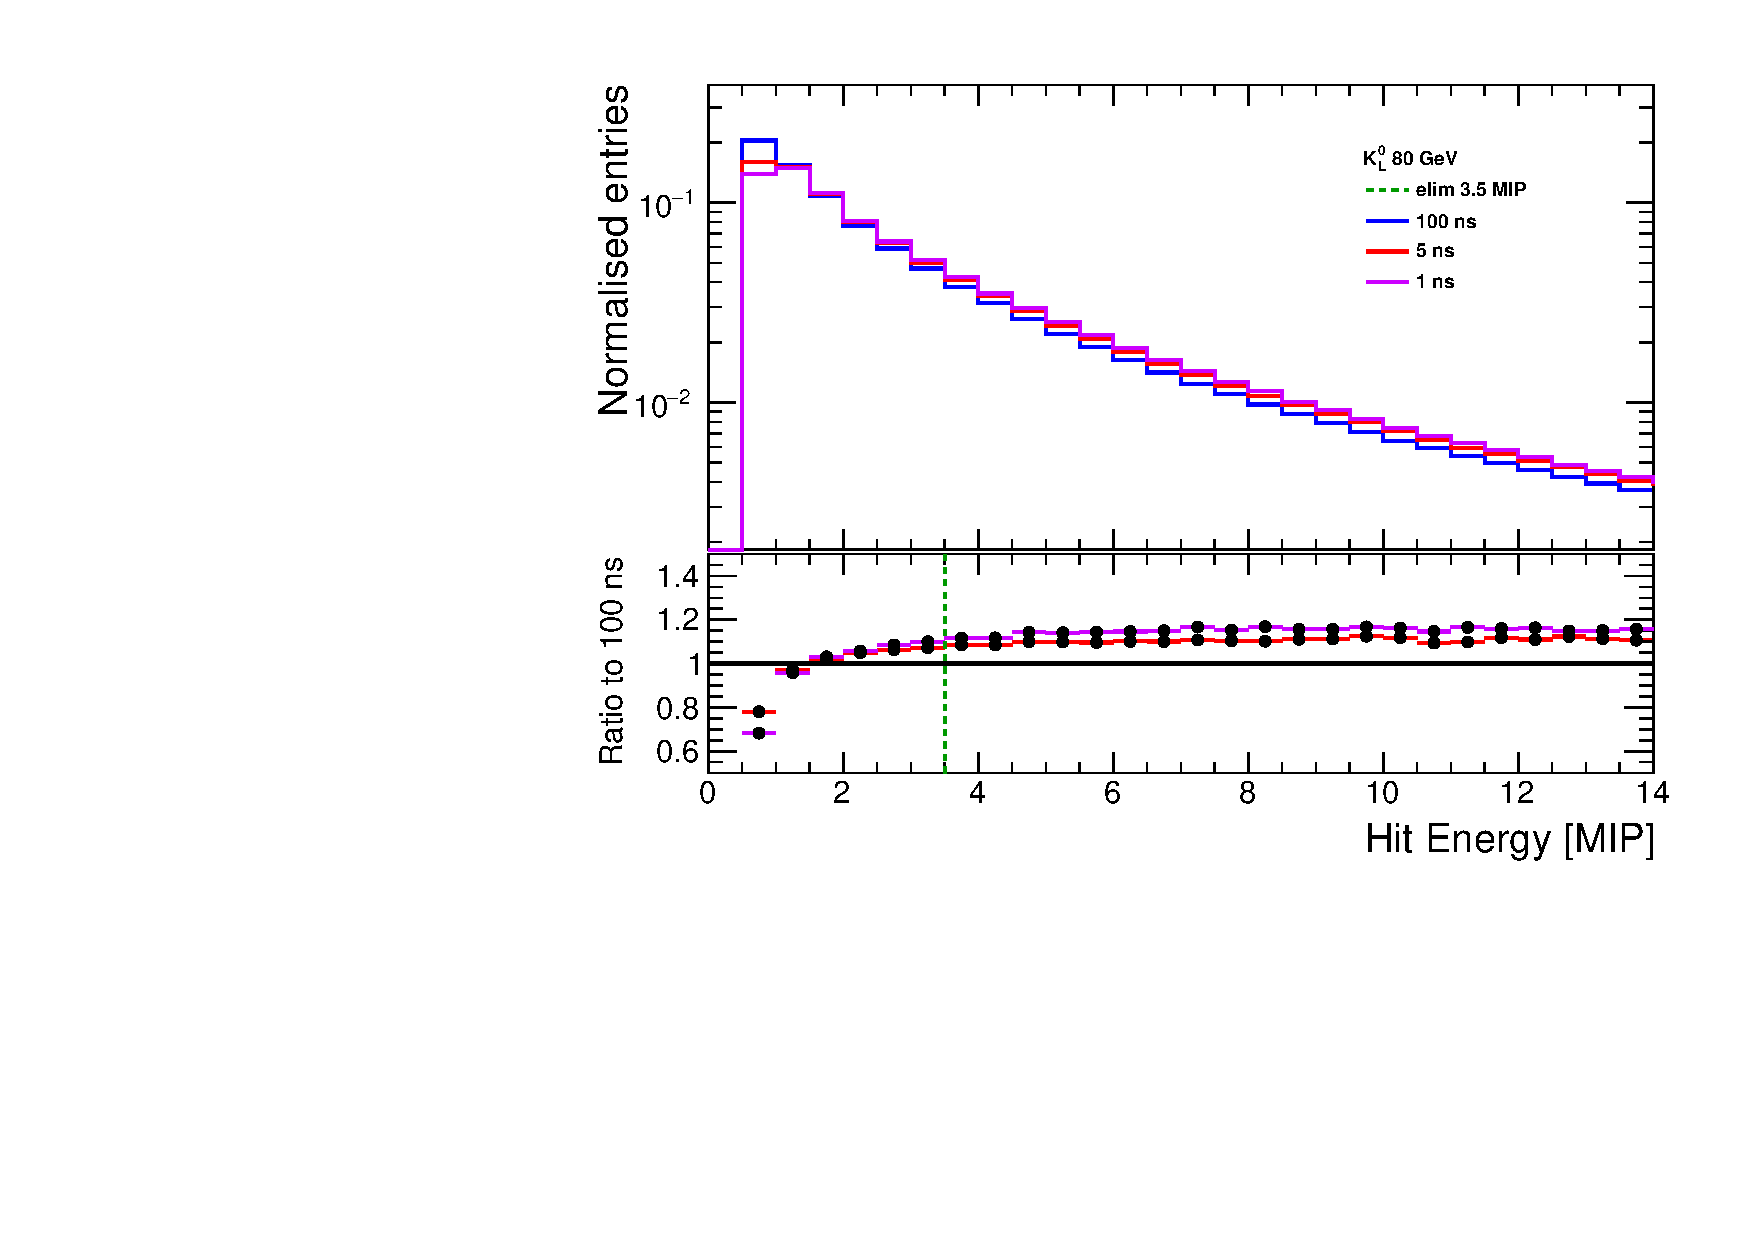
\includegraphics[width=0.7\linewidth]{../Thesis_Plots/ILD/AdditionalPlots/Plots/HitEnergySpectra_80GeV.pdf}
  \caption{The top plots shows the hit energy spectra in the HCAL for 80 GeV kaons with different timing cuts applied. The bottom plot shows the ratio of the spectra compared to 100 ns.} \label{fig:HitSpectra80_timingcuts}
\end{figure}

One can notice that the shape of the spectra differs slightly with timing cuts, a reduction of low energy hits (~ 1 MIP) and a higher tail to higher hit energies. With a cut of 1 ns, there are around 10\% more hits over 4 MIPs. With a value of 3.5 MIP for $e^{lim}$, it seems that there are globally fewer hits below, thus reducing the value of $C^{lim}$ ($C^{av}$ is quite independent of the timing cut). A lower value of $C^{lim}$/$C^{av}$ corresponds to a higher energy deposited thus giving a hint that timing cuts enhance the electromagnetic response of the calorimeter making even more non-compensating. To further confirm this observation, the same correlation plots between the energy deposited in the HCAL and the ratio $C^{lim}$/$C^{av}$ is shown in figures \ref{fig:EhcalCLimCav10_1ns} and \ref{fig:EhcalCLimCav80_1ns}.

\begin{figure}[htbp!]
  \centering
  \begin{subfigure}[t]{0.45\textwidth}
    \centering
    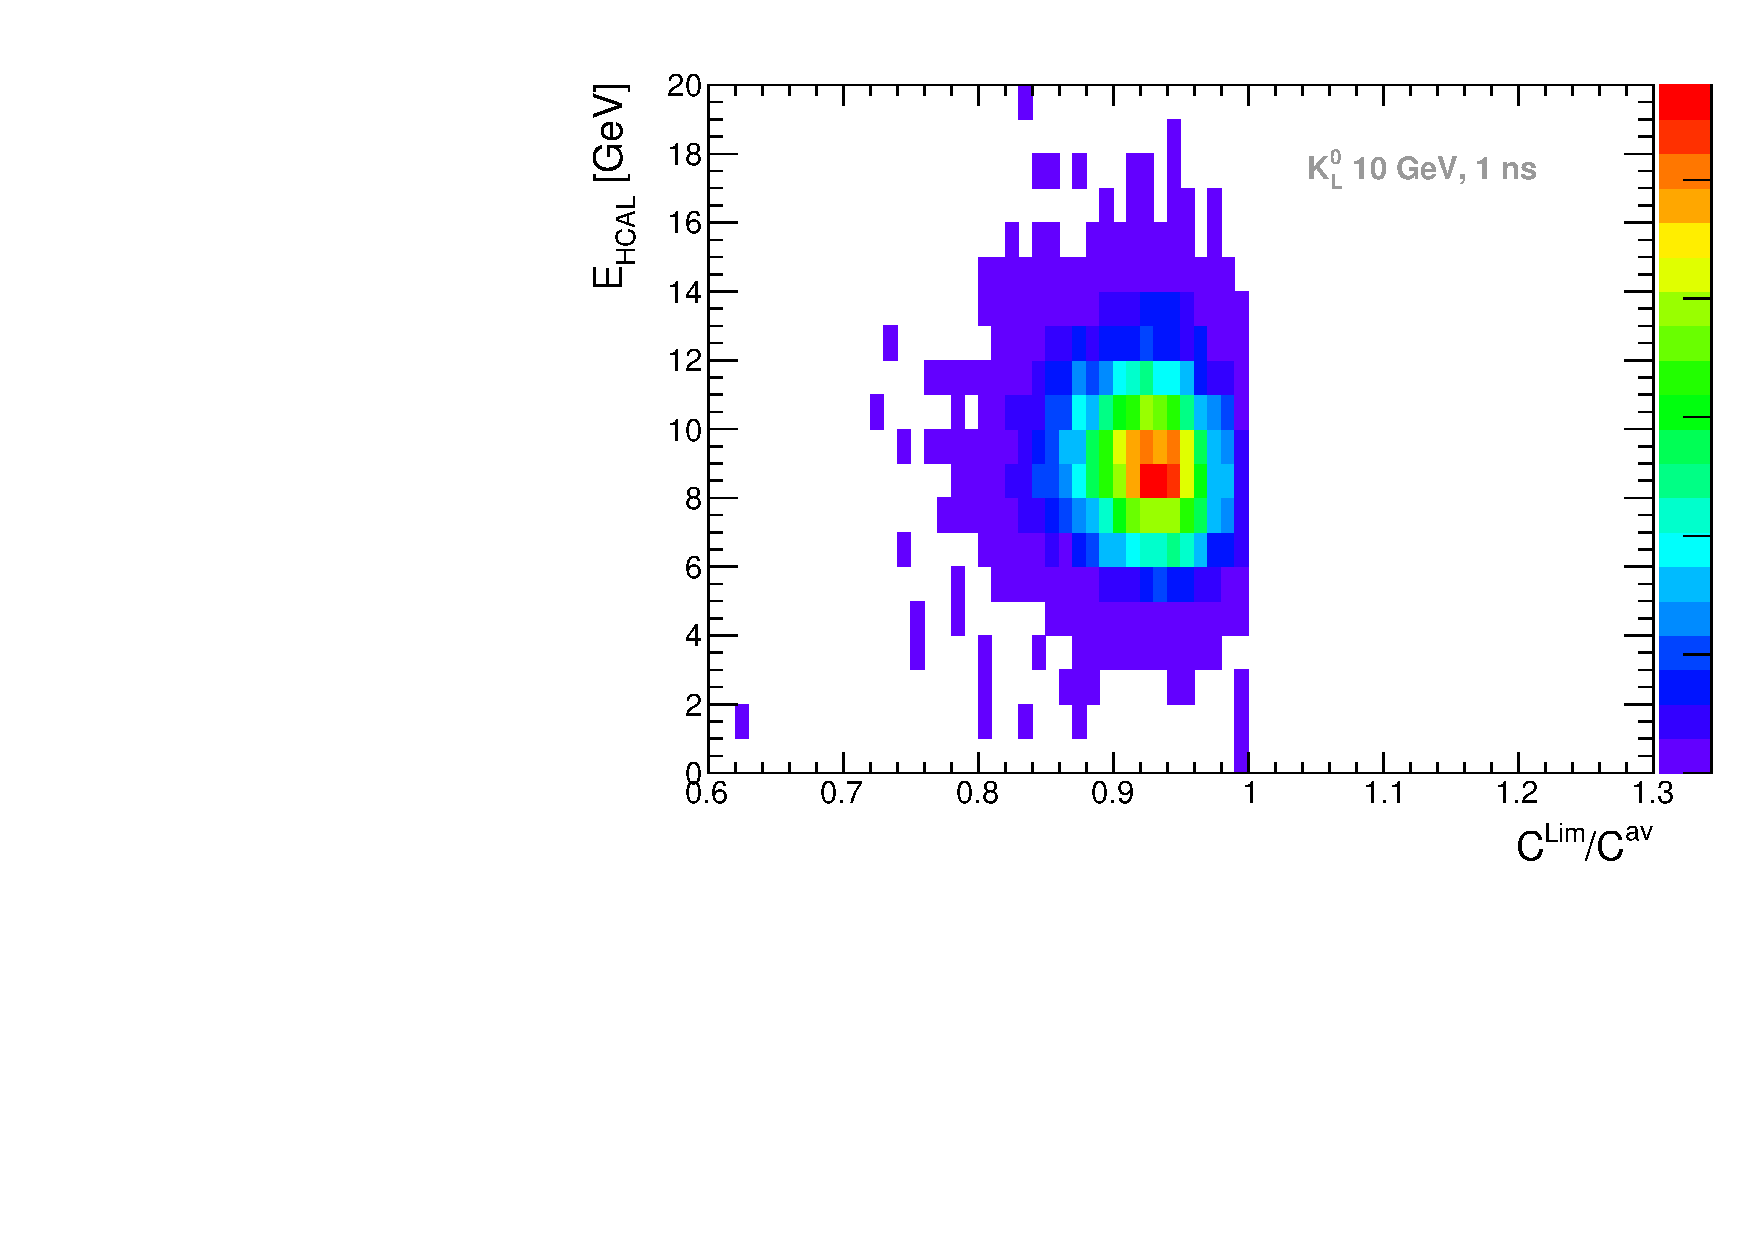
\includegraphics[width=1\linewidth]{../Thesis_Plots/ILD/AdditionalPlots/Plots/EhcalCLimCav_1ns_10GeV.pdf}
    \caption{10 GeV.} \label{fig:EhcalCLimCav10_1ns}
  \end{subfigure}
  \hfill
  \begin{subfigure}[t]{0.45\textwidth}
    \centering
    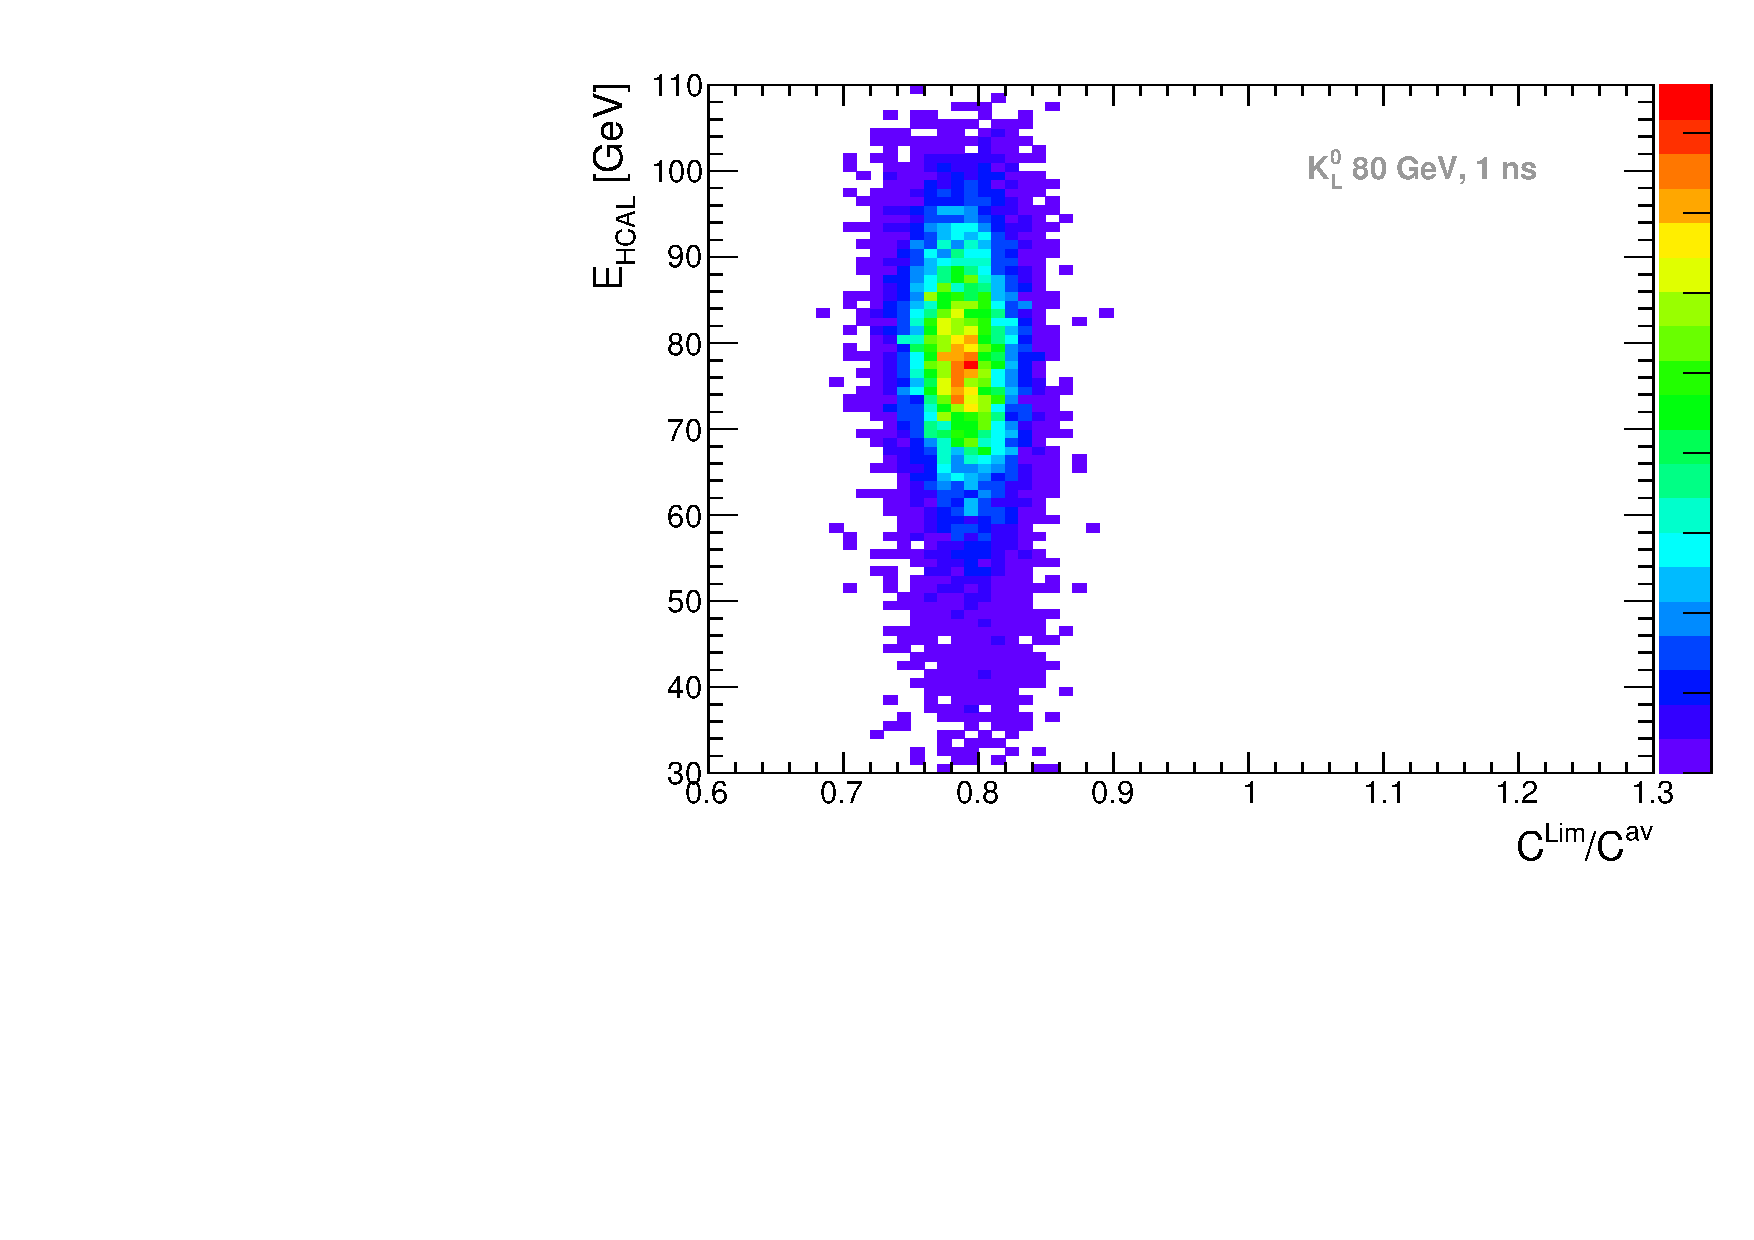
\includegraphics[width=1\linewidth]{../Thesis_Plots/ILD/AdditionalPlots/Plots/EhcalCLimCav_1ns_80GeV.pdf}
    \caption{80 GeV.} \label{fig:EhcalCLimCav80_1ns}
  \end{subfigure}
  \caption{\subref{fig:EhcalCLimCav10_1ns}) Correlation between the energy deposited in the HCAL for 10 GeV kaons and $C^{lim}$/$C^{av}$ for $e^{lim}$ = 3.5 MIPs with a timing cut of 1 ns. \subref{fig:EhcalCLimCav80_1ns}) Correlation between the energy deposited in the HCAL for 80 GeV kaons and $C^{lim}$/$C^{av}$ for $e^{lim}$ = 3.5 MIPs with a timing cut of 1 ns.}
\end{figure}

It appears that the anti-correlation is reduced slightly but more visible for lower energy kaons. This further confirms that the timing cuts reduce the fluctuations between the electromagnetic and hadronic fractions in hadronic showers by cutting the hadronic response and enhancing the electromagnetic one. This has an effect of non-compensation in the response to hadronic showers thus degrading the energy resolution furthermore.
